% Template for PLoS
% Version 1.0 January 2009
%
% To compile to pdf, run:
% latex plos.template
% bibtex plos.template
% latex plos.template
% latex plos.template
% dvipdf plos.template

\documentclass[10pt]{article}

% amsmath package, useful for mathematical formulas
\usepackage{amsmath}
% amssymb package, useful for mathematical symbols
\usepackage{amssymb}

% graphicx package, useful for including eps and pdf graphics
% include graphics with the command \includegraphics
\usepackage{graphicx}

% cite package, to clean up citations in the main text. Do not remove.
\usepackage{cite}

\usepackage{color} 

% Use doublespacing - comment out for single spacing
\usepackage{setspace} 
\doublespacing

\usepackage{multirow}

% Text layout
\topmargin 0.0cm
\oddsidemargin 0.5cm
\evensidemargin 0.5cm
\textwidth 16cm 
\textheight 21cm

% Bold the 'Figure #' in the caption and separate it with a period
% Captions will be left justified
\usepackage[labelfont=bf,labelsep=period,justification=raggedright]{caption}

% Use the PLoS provided bibtex style
\bibliographystyle{plos2009}

% Remove brackets from numbering in List of References
\makeatletter
\renewcommand{\@biblabel}[1]{\quad#1.}
\makeatother


% Leave date blank
\date{}

\pagestyle{myheadings}
%% ** EDIT HERE **


%% ** EDIT HERE **
%% PLEASE INCLUDE ALL MACROS BELOW

%% END MACROS SECTION

\begin{document}

% Title must be 150 characters or less
\begin{flushleft}
{\Large
\textbf{mRNA-Seq Assembly Discovers Many Novel Splice Variants}
}
% Insert Author names, affiliations and corresponding author email.
\\
Likit Preeyanon$^{1}$, 
Jerry B. Dodgson$^{1}$
Hans Cheng$^{2}$, 
C. Titus Brown$^{3,1 \ast}$
\\
\bf{1} Microbiology and Molecular Genetics, Michigan State University, East Lansing, MI, USA.
\\
\bf{2} Avian Disease and Oncology Laboratory, East Lansing, MI, USA.
\\
\bf{3} Department of Computer Science and Engineering, Michigan State University, East Lansing, MI, USA.
\\
$\ast$ E-mail: ctb@msu.edu
\end{flushleft}

% Please keep the abstract between 250 and 300 words
\section*{Abstract}

% Please keep the Author Summary between 150 and 200 words
% Use first person. PLoS ONE authors please skip this step. 
% Author Summary not valid for PLoS ONE submissions.   
\section*{Author Summary}

\section*{Introduction}

% Results and Discussion can be combined.
\section*{Results}

\subsection*{Transcripts from Global and Local Assembly}
\subsubsection*{Different Isoforms Detected by Different k-mers}

Without high quality annotations, it is necessary that we construct gene models containing putative isoforms to identify alternative splicing in our samples.
We used Velvet\cite{Zerbino:2008vu} and Oases assembler to construct transcripts from short reads.
We ran Velvet using default settings except a hash length or k-mer parameter, which has no default values.
To find an appropriate value for hash length for our datasets, we experimented on a wide range of k-mer lengths from 23 to 35.
After comparing transcripts from all k-mers, we found that some isoforms were only detected in some particular k-mers (Fig.~\ref{figure4}).
Therefore, instead of choosing one k-mer, we ran Velvet assembler with multiple k-mers and combined the results to increase sensitivity of isoform detection.

\subsubsection*{Local Assembly Enhances Isoform Detection}

Performing assembly with multiple k-mers is time and memory consuming.
To facilitate this, we partitioned reads into groups based on their alignments to the chicken genome.
We refer to this method as a local assembly and a conventional assembly method as a global assembly in this study (see materials and methods).
The advantages of the local assembly method are that each group of reads can be assembled using small amount of memory and it can be assembled on different computers.
Furthermore, we found that local assembly could identify unique alternative splicing from global assembly.
Therefore, we performed both global and local assembly with multiple k-mers (23-35 and 15-39 respectively) to obtain all possible alternative splicing detected from both methods.
Figure~\ref{figure5} shows an example of isoforms detected with different k-mers in two assembly methods.

Using global and local assembly methods, we obtained a different number of contigs.
Table 1 shows a number of contigs from four datasets and unique contigs from global and local assemblies.
As expected, some sequences from local assembly (0.5--0.7\%) are not detected in global assembly.
Homology search in mouse proteins showed that 4--5.6\% of unique regions from local assembly are genuine protein coding sequences (Table 2).
This suggests that some isoforms will be missing in the gene models based solely on global assembly.
In addition, a significant number of transcripts from global assembly are unique, which indicates that approximately 4.8\% of coding sequences are missing in a current chicken genome.

\subsection*{Predicted Gene Models from Assembly}

All transcripts were assembled by Gimme to construct gene models.
Total of 27,448 multi-exon genes were obtained from global assembly and 22,434 genes from local assembly.
However, the number of genes obtained from global + local assembly is only 32,854.
This indicates that some transcripts from both methods were common or merged together.
As expected, the number of genes and isoforms increased significantly after combining global and local assembly together due to the increased number of splice junctions (Table 3). 
      
\subsection*{Fragmented transcripts}
The number of genes from our pipeline is unexpectedly high due to a large number of two-exon genes. As shown in Table 3, the number of two-exon genes is high (28-34\% in models derived from assembly), compared to the number of annotated two-exon genes in reference genes (6\%).
The majority of two-exon genes are shorter than 500bp as shown in Fig.~\ref{figure7}.
Homology search against mouse proteins (using blastp) showed that 60\% of two-exon genes that matched mouse proteins are shorter than 500bp (Fig.~\ref{figure8}).
The results suggest that these two-exon genes are indeed genuine coding sequences.
However, according to their small size, they are possibly parts of larger transcripts that were not completely assembled.
In our datasets, read coverage is lower at the $5'$ end due to the method used to converse mRNA to cDNA in sequencing.
A bias of read coverage toward $3'$ end and low expression level result in fragmented transcripts as shown in Fig.~\ref{figure9}.
Notably, the number of two-exon genes decreased when reference genes were incorporated to global + local assembly gene models (Table 3).
This indicates that some two-exon genes were merged to reference genes since they are part of larger transcripts.

\subsection*{Characteristics of RNA-Seq Derived Gene Models}
Gene models derived from our pipeline are comparable or, in some cases, more complete than gene models available on UCSC genome browser\cite{ucscGenomeBrowser}.
Fig.~\ref{figure10} shows a comparison of a predicted isoforms with gene models from reference genes, Ensembl[?], N-SCAN[?] and Genscan[?].
Our gene models have an advantage of including extended untranslated regions (UTRs), especially $3'$ UTR in our datasets.
These regions are challenging to predict correctly solely from computational methods due to low degree of conservation [?].
RNA-Seq-derived gene models will facilitates the detection of variations within UTR regions, which may be involved in regulating the expression of the isoform [?] (Fig.~\ref{figure11}).

\subsection*{Comparison with Cufflinks and Trinity}
To evaluate an efficiency of our pipeline in detecting splice junctions,
we compared the number of splice junctions detected by our pipeline to those from Cufflinks\cite{Trapnell:2010kd} and Trinity\cite{Grabherr:2011jb}.
Cufflinks detected 99,958 (85\%) splice junctions that are also detected by our pipeline (Fig.~\ref{figure17}).
60,849 (37.8\%) are not detected by Cufflinks of which 29,207 (48\%) are supported by at least four spliced reads.

Reads from line 6 uninfected dataset that mapped to a chromosome 1 were assembled using Trinity with default settings.
Trinity found a total of 11,902 splice junctions; whereas, our pipeline detected 12,676 splice junctions.
1,395 splice junctions are not found by Trinity and 621 junctions are not detected by our pipeline.
Figure~\ref{figure19} summarizes a number of splice junctions in chromosome 1 detected by all three methods.
Figure~\ref{figure20} shows two splice variants that are detected by local assembly but not Trinity.

\subsection*{Validation of Gene Models}

The results show that our pipeline can be used to detect alternative splicing and construct gene models from a large set of transcripts from assembly.
However, many steps in our pipeline can introduce errors to the gene models.
We performed several methods to validate the gene models as described below.

\subsubsection*{Reads Mapped to Gene Models}

Single-end reads from the same datasets that we used to build the gene models were aligned to the DNA sequences derived from the gene models.
We anticipated that a large number of reads could align to the gene models.
We found that 66-73\% of reads mapped to the gene models (Table 4).
In addition, we mapped paired-end reads that we obtained later from the same samples to the gene models and found that more than 60\% of reads mapped to the gene models (Table 5).
The results suggest that the gene models are of high quality.

\subsubsection*{Conserved Reading Frame}
Alternative isoforms usually maintain a reading frame to be functional [?].
We hypothesized that errors in our pipeline that introduce false splice junctions will disrupt the reading frame.
Although, in nature, alternative-splicing events can disrupt the reading frame, we expected a significant number of isoforms to be translatable. 

Transcripts from RNA-Seq assembly are supposed to contain UTRs and coding sequences. However, due to some factors mentioned previously, we could not obtain complete transcripts for all isoforms.
Thus, predicting the reading frame or coding sequence solely from sequence signals is not feasible.
We used ESTScan\cite{Iseli:1999vd}, a program that is designed to find coding sequences from expressed sequence tags (ESTs) and does not rely on sequence signals to translate isoforms to protein sequences.
To evaluate the result, we used reference mRNAs as a control.
However, since our gene models derived from the chicken genome sequence; therefore, we first aligned reference mRNAs to the genome to obtain DNA sequences to be used in the comparison.

ESTScan successfully translated 47,786 (80\%) isoforms from our gene models and 15,952 and 14,999 (97\%) sequences from reference mRNAs and models built from reference mRNAs.
We evaluated the completeness of coding sequence by comparing the number of nucleotides in each isoform to the number of amino acid encoding nucleotides.
We found that cumulative distributions of ratios from reference mRNAs before and after processed by our pipeline are highly similar.
This indicates that the pipeline did not introduce errors that disrupt the reading frame of the mRNAs.
The result from our gene models shows significant similarity to results from mRNAs, which suggests that a majority of isoforms detected by our pipeline is translatable.

\subsubsection*{Homologous sequences in mouse}
To further examine quality of protein sequences derived from our gene models, we searched for homologous sequences in mouse \textit{(Mus musculus)}, which is a related and well-studied animal.
We found 29,903 (52\%) isoforms (7,425 genes) match mouse proteins.
As shown in Fig.~\ref{figure14}, most genes and isoforms have a bit score/length ratio more than 1.0, which indicates a good agreement between chicken and mouse proteins.
The results illustrate that isoforms constructed by our pipeline are translatable and may be functional.
However, genes or isoforms with no match to mouse proteins are not necessarily artifacts.
They can be genes or isoforms that are only found in other vertebrates or novel genes.

\subsubsection*{Reads mapped to splice junctions}
We identified 160,807 splice junctions from the gene models.
To validate the splice junctions, we mapped reads to DNA sequences derived from gene models using Bowtie\cite{Langmead:2009fv}.
Because the mapping algorithm implemented in Bowtie does not consider splice sites, reads mapped across splice junctions confirm that the splice junctions are real.
Of all spliced junctions, 18,004 (11\%) junctions have no spliced reads and 11,815 (6.9\%) junctions have 1--3 spliced reads (see materials and methods).
This demonstrates that the method detects splice junctions with high specificity.
Splice junctions with fewer than four spliced reads, however, may not be considered false junctions because of a bias of read coverage toward $3'$ end in our datasets.
Reads are less abundant at the $5'$ end of transcripts; therefore, a relatively small number of spliced reads mapped to splice junctions near the $5'$ end.

\section*{Discussion}

In this study, we used multiple k-mers and a local assembly method to enhance splice variant detection.
Our new method detects splice variants that are not detected by a conventional assembly method.
We also showed that our method can be used with other programs (Cufflinks, Trinity, etc.) to increase sensitivity of splice variant detection.
It works well with single-ended reads and does not require more memory than the conventional assembly method.
The method, however, relies on a quality of a reference genome and a read mapping program.

We also presented Gimme, a program that assembles transcripts from different approaches based on alignments to a reference genome to construct gene models.
We used the pipeline to construct gene models from chicken mRNAs using global and local assembly to identify novel genes and isoforms in chicken.
Many novel genes and isoforms are found and validation results suggest that a majority of them are genuine and may be of biological importance.
The gene models also markedly improve existing annotations.

% You may title this section "Methods" or "Models". 
% "Models" is not a valid title for PLoS ONE authors. However, PLoS ONE
% authors may use "Analysis" 
\section*{Materials and Methods}

\subsection*{Mapping reads to The Reference Genome and Gene Models}

Single and paired-end reads were mapped to chicken genome by Tophat\cite{Trapnell:2009dp} version 1.0.13 using default parameters without annotations.
All reads were mapped to DNA sequences derived from gene models by Bowtie version 0.12.7\cite{Langmead:2009fv} with default parameters \texttt{(n=2, l=28, e=70, k=1)}.

\subsection*{Global and Local Assembly}

Reads from each dataset were first assembled separately in global assembly without using a reference genome.
In contrast, reads from each dataset were first mapped to the chicken genome using Tophat.
Then only reads that mapped to the genome were assembled by chromosomes in local assembly (Fig.~\ref{figure1}).
Global and local assembly was performed using Velvet version 1.0.17\cite{Zerbino:2008vu} with default parameters except for hash length (k-mer).
k-mer lengths ranging from 15 to 39 were used in local assembly and from 23 to 35 in global assembly to increase sensitivity of splice junction detection.
Lastly, transcripts from both methods were assembled by Oases version 0.1.18 (unpublished).

\subsection*{Gene Model Construction}

\subsubsection*{Overall Pipeline}

Transcripts of all datasets from local and global assembly were mapped to the chicken genome using GMAP version 2011-03-28.v3\cite{Wu:2005bl} \texttt{(-n 0)}.
Alignments and gaps from GMAP outputs are considered exons and introns respectively.
Optionally, data from other sources (ESTs, RefGenes, etc.) can be incorporated with transcripts from assembly to improve gene models.
All transcripts are then assembled using Gimme, a program that assembles transcripts based on their alignments to the reference genome.
An algorithm for assembling transcripts is described below.

\subsubsection*{Algorithm}

A gene model can be represented as a splice graph composed of exons as nodes and introns as edges.
However, transcripts of the same gene vary in size and structure depending on the expression level and a hash length number used in assembly.
Furthermore, incomplete exons and fragmented transcripts complicate the construction of a splice graph.
In this study, we developed an algorithm that handles incomplete exons and fragmented transcripts and constructs a maximum assembly of gene models.

The algorithm first builds an intron graph using introns as nodes  (Fig.~\ref{figure3}).
Each intron contains exons whose one of their splice sites perfectly match intron boundary.
Exons are considered incomplete and eliminated if they locate at the $3'$ or $5'$ end of the transcripts and they are not the largest exons (exon 3a and 3b in Fig.~\ref{figure3}).
Transcripts were then grouped into the same gene if they have at least one intron or exon in common (Fig.~\ref{figure3}).
Then, a splice graph composed of exons is created and structures of isoforms are derived from traversing paths in the splice graph.
Two sets of putative transcripts can be constructed --- a maximum and a minimum set.
The maximum set contains all putative isoforms, which are derived from all paths in splice graphs.
In contrast, the minimum set contains minimum isoforms that represents all unique edges in splice graphs.

\subsection*{Open Reading Frame and Strand Prediction}

We employed ESTScan version 2.1\cite{Iseli:1999vd} to predict strand and ORFs for our gene models.
The matrix used for building Hidden Markov model was built from chicken reference cDNA sequences using tools from ESTScan.

\subsection*{Finding Unique Sequences Between Datasets}

To identify unique sequences from two datasets, a set of 20-mers is created for both datasets using khmer [?].
Then, 20-mers from a query dataset are compared with 20-mers from the target dataset.
The sequence is considered unique if more than 90\% of 20-mers in the query is unique.
Any unique region shorter than 100bp is ignored.

\subsection*{Sequence Homology Analysis}

Protein sequences translated from each isoform using ESTScan were searched against mouse reference sequences [?] by BLAST 2.2.25+\cite{Tatusova:1999tz}.
A bit score to a length ratio was calculated for each hit that had e-value $\le 10^{-20}$.
Only the highest ratio of all isoforms of a gene was used in the gene-wise analysis, whereas, all ratios were used in the isoform-wise analysis.

\subsection*{Spliced Reads Counting}

Reads from each dataset were mapped to transcripts from the gene models using Bowtie version 0.12.7 using default parameters.
Only reads that mapped across exon junctions from all datasets were counted using Samtools\cite{Li:2009vz} and Pysam [?]

\subsection*{Sequence Assembly using Trinity}
To be added.

\subsection*{Sequence Assembly using Cufflinks}
To be added.

% Do NOT remove this, even if you are not including acknowledgments
\section*{Acknowledgments}

Royal Thai Government Scholarship.

{\noindent}USDA funding.

%\section*{References}
% The bibtex filename
\bibliography{refs}

\section*{Figure Legends}
\begin{figure}[!ht]
\begin{center}
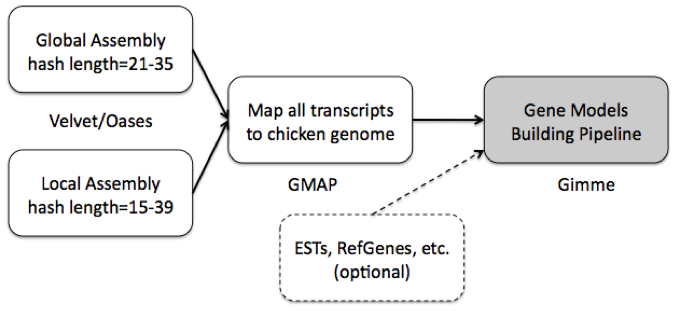
\includegraphics[width=5in]{figure1.png}
\end{center}
\caption{
{\bf Gene model construction pipeline.} Transcripts are obtained from two assembly methods -- global and local assembly.
Transcripts are aligned to a chicken genome by GMAP. Gimme then constructs gene models based on alignments of transcripts.
}
\label{figure1}
\end{figure}

\begin{figure}[!ht]
\begin{center}
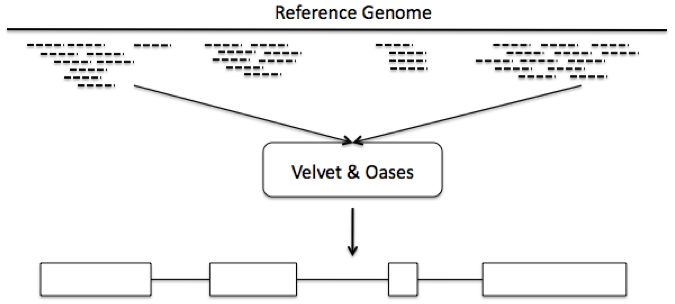
\includegraphics[width=5in]{figure2.png}
\end{center}
\caption{
{\bf Local Assembly Pipeline.}
Reads are first mapped to a chicken genome.
Then only mapped reads are assembled by Velvet and Oases.
}
\label{figure2}
\end{figure}

\begin{figure}[!ht]
\begin{center}
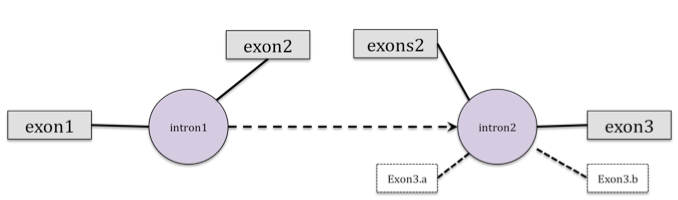
\includegraphics[width=5in]{figure3a.png}
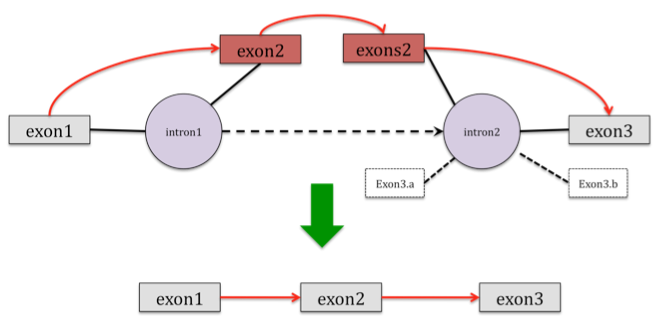
\includegraphics[width=5in]{figure3b.png}
\end{center}
\caption{
{\bf Intron and exon graphs.}
a. Each intron connects to exons whose splice junctions match it boundary.
Some exons are excluded from the final gene model if they are incomplete.
b. Introns sharing at least one exon are grouped together.
Then an exon graph is made using exons as nodes.
}
\label{figure3}
\end{figure}

\begin{figure}[!ht]
\begin{center}
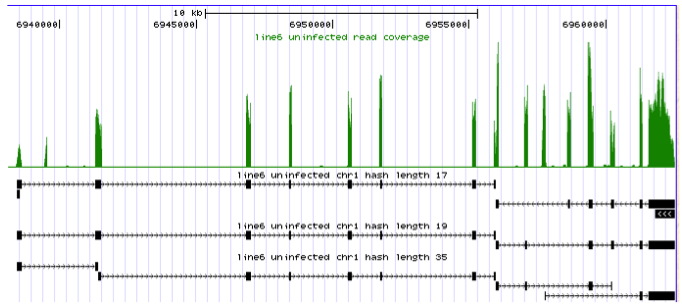
\includegraphics[width=5in]{figure4.png}
\end{center}
\caption{
{\bf Different isoforms are detected by different k-mer lengths.}
}
\label{figure4}
\end{figure}

\begin{figure}[!ht]
\begin{center}
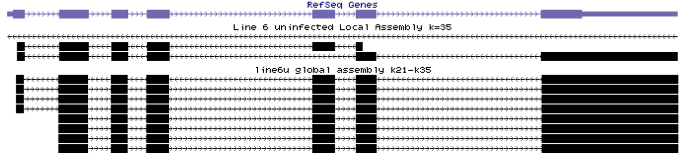
\includegraphics[width=5in]{figure5.png}
\end{center}
\caption{
{\bf Global and local detect different isoforms with the same k-mers.} 
}
\label{figure5}
\end{figure}

\begin{figure}[!ht]
\begin{center}
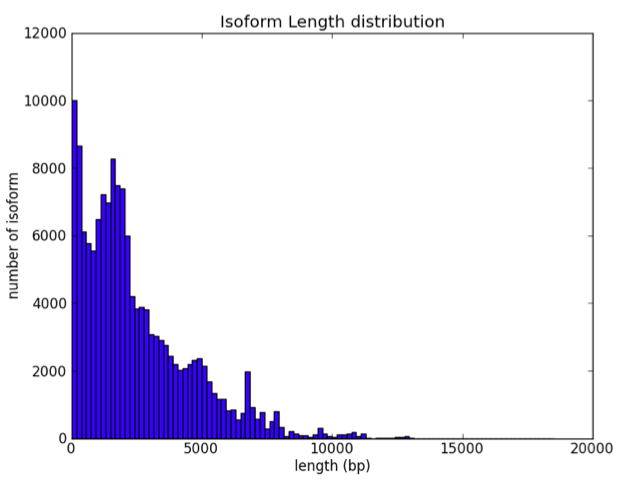
\includegraphics[width=5in]{figure6.png}
\end{center}
\caption{
{\bf Isoform length distribution.} 
}
\label{figure6}
\end{figure}

\begin{figure}[!ht]
\begin{center}
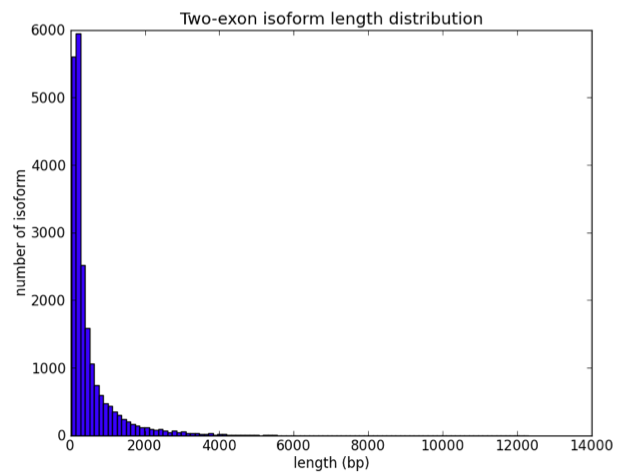
\includegraphics[width=5in]{figure7.png}
\end{center}
\caption{
{\bf Isoform length distribution of two-exon transcripts.} 
}
\label{figure7}
\end{figure}

\begin{figure}[!ht]
\begin{center}
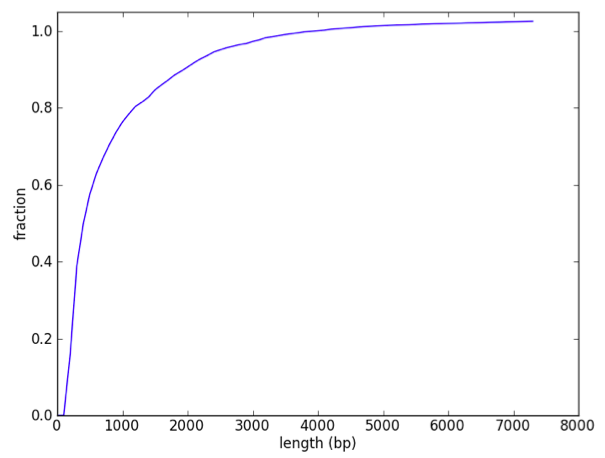
\includegraphics[width=5in]{figure8.png}
\end{center}
\caption{
{\bf Cumulative distribution of lengths of two-exon transcripts homologous to mouse proteins.}
}
\label{figure8}
\end{figure}

\begin{figure}[!ht]
\begin{center}
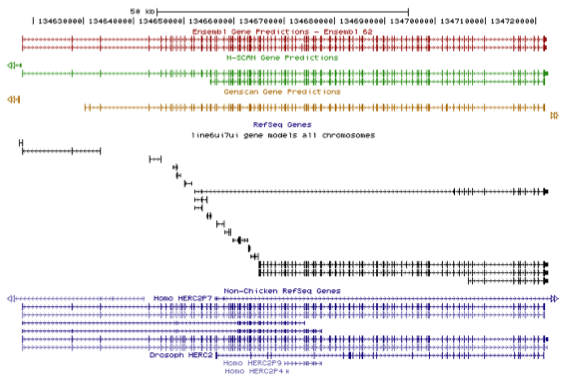
\includegraphics[width=5in]{figure9.png}
\end{center}
\caption{
{\bf Example of fragmented transcripts near $5'$ end of a long transcript.}
}
\label{figure9}
\end{figure}

\begin{figure}[!ht]
\begin{center}
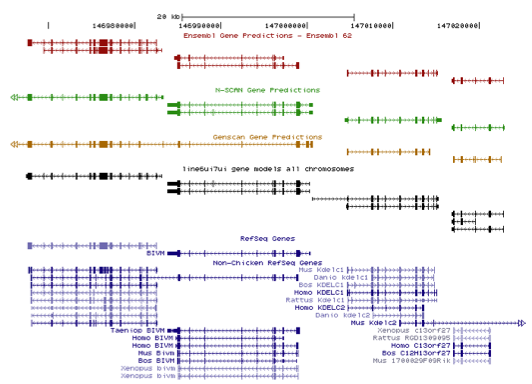
\includegraphics[width=5in]{figure10.png}
\end{center}
\caption{
{\bf Comparison of RNA-Seq derived gene models and other publicly available gene models from UCSC genome browser.}
}
\label{figure10}
\end{figure}


\begin{figure}[!ht]
\begin{center}
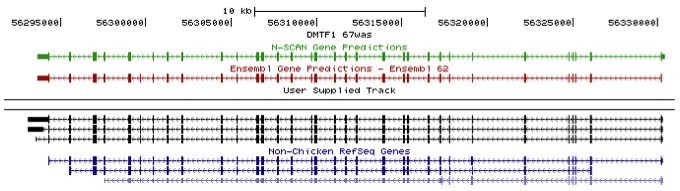
\includegraphics[width=5in]{figure11.png}
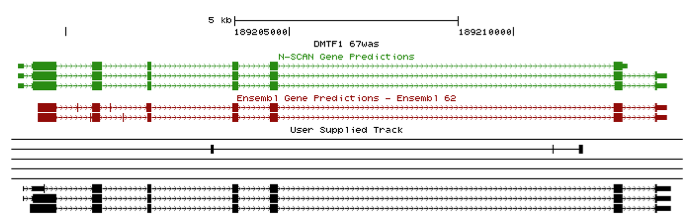
\includegraphics[width=5in]{figure12.png}
\end{center}
\caption{
{\bf Examples of alternative $3'$ and $5'$ UTRs detected in RNA-Seq gene models.}
}
\label{figure11}
\end{figure}

\begin{figure}[!ht]
\begin{center}
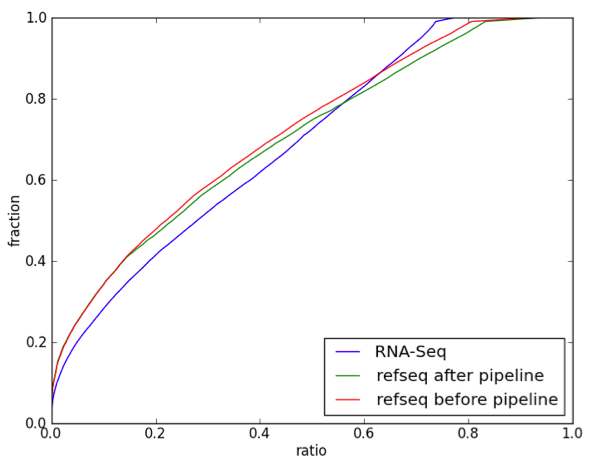
\includegraphics[width=5in]{figure13.png}
\end{center}
\caption{
{\bf Cumulative distribution of the ratio of the number of nucleotides to the number of amino acid encoding nucleotides.}
}
\label{figure13}
\end{figure}

\begin{figure}[!ht]
\begin{center}
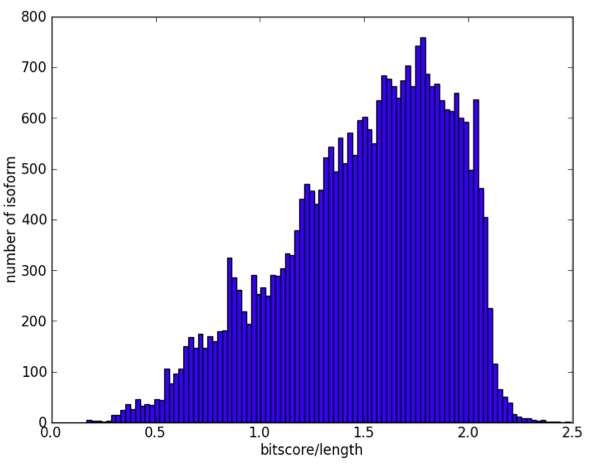
\includegraphics[width=5in]{figure14.png}
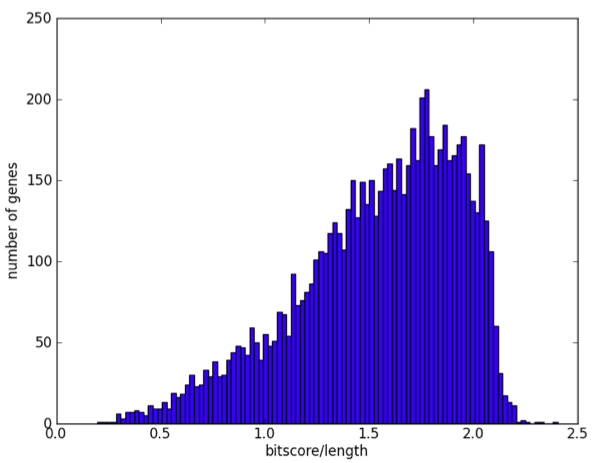
\includegraphics[width=5in]{figure15.png}
\end{center}
\caption{
{\bf Histogram of bit score/length ratio of isoforms and genes that match mouse proteins.}
}
\label{figure14}
\end{figure}

\begin{figure}[!ht]
\begin{center}
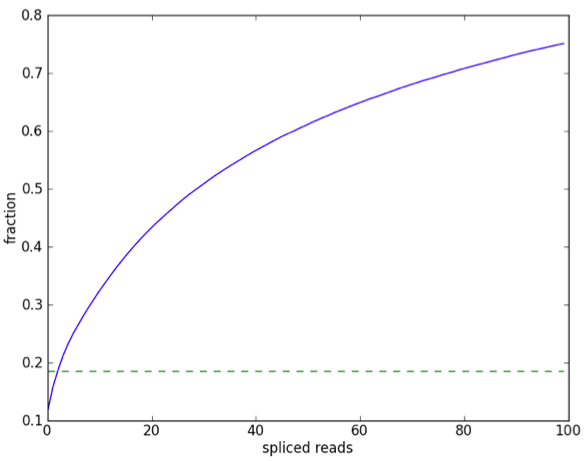
\includegraphics[width=5in]{figure16.png}
\end{center}
\caption{
{\bf Cumulative counts of splice junctions with spliced reads.}
}
\label{figure16}
\end{figure}

\begin{figure}[!ht]
\begin{center}
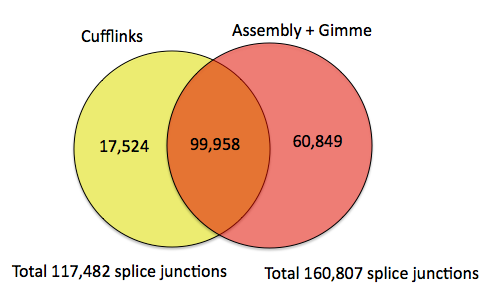
\includegraphics[width=5in]{figure17.png}
\end{center}
\caption{
{\bf Splice junctions found by Cufflinks and Gimme.}
}
\label{figure17}
\end{figure}

\begin{figure}[!ht]
\begin{center}
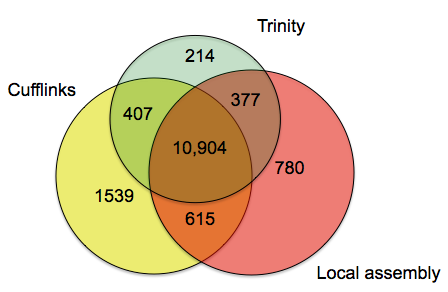
\includegraphics[width=5in]{figure19.png}
\end{center}
\caption{
{\bf Number of splice junctions in chromosome 1 detected by local assembly, Cufflinks and Trinity.}
}
\label{figure19}
\end{figure}

\begin{figure}[!ht]
\begin{center}
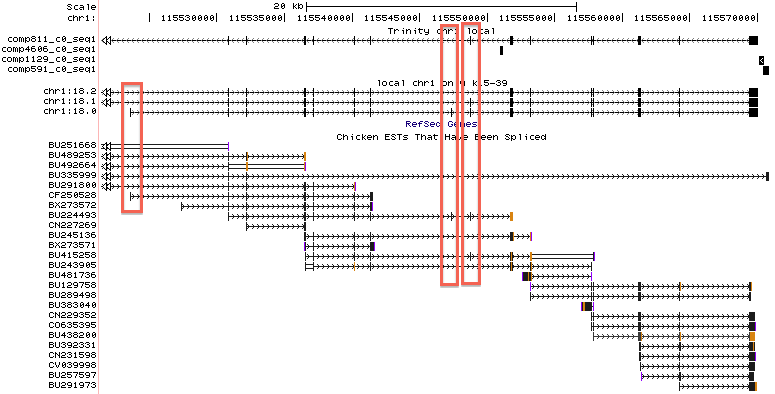
\includegraphics[width=7in]{figure20.png}
\end{center}
\caption{
{\bf Example of splice variants detected by local assembly but not Trinity.}
Local assembly detects two exons that are not detected by Trinity.
These two exons are included in a shorter isoform of this gene and are supported by ESTs.
Local assembly also detects another isoform that contains a skipped exon, which is also supported by ESTs.
}
\label{figure20}
\end{figure}

\section*{Tables}
\begin{table}[!ht]
\caption{
\bf{Unique sequences from global and local assembly}}
\begin{tabular}{ccccc}
\hline
Dataset & \multicolumn{2}{c}{Total Sequence} & \multicolumn{2}{c}{Unique Sequence}\\
 & Global & Local & Global & Local\\
\hline
Line 6 uninfected & 486,151 & 628,811 & 17,961 (3.6\%) & 3,563 (0.05\%)\\
Line 6 infected & 389,854 & 572,672 & 18,852 (4.8\%)& 4,107 (0.07\%)\\
Line 7 uninfected & 445,017 & 584,037 & 16,432 (3.6\%) & 3,991 (0.07\%)\\
Line 7 infected & 510,059 & 631,081 & 20,321 (3.9\%)& 3,649 (0.06\%)\\
\hline
%table information
\end{tabular}
%\begin{flushleft}Table Caption
%\end{flushleft}
%\label{tab:label}

\caption{
\bf{Unique regions from global and local assembly}}
\begin{tabular}{ccccc}
\hline
Dataset & \multicolumn{2}{c}{Unique Region} & \multicolumn{2}{c}{Matched with mouse proteins}\\
 & Global & Local & Global & Local\\
\hline
Line 6 uninfected & 19,084 & 4,685 & 3,113 (16\%) & 194 (4\%)\\
Line 6 infected & 20,003 & 6,177 & 3,730 (19\%)& 224 (3.6\%)\\
Line 7 uninfected & 17,564 & 5,655 & 2,864 (16\%) & 320 (5.6\%)\\
Line 7 infected & 21,384 & 4,894 & 2,832 (13\%)& 238 (4.8\%)\\
\hline
%table information
\end{tabular}
%\begin{flushleft}Table Caption
%\end{flushleft}
%\label{tab:label}

\caption{
\bf{Number of putative genes and isoforms}}
\begin{tabular}{cccccc}
\hline
Method& Gene & \multicolumn{4}{c}{Isoform} \\ 
& & Maximum & Minimum & Multiexon* & Two-exon* \\
\hline
Global & 27,448 & 65,376 & 42,375 & 27,891 & 14,484 (34\%) \\
Local & 22,434 & 82,285 & 38,876 & 27,724 & 11,152 (28\%) \\
Global + Local & 32,854 & 196,024 & 59,430 & 39,570 & 19,860 (33\%) \\
RefGenes & 4,567 & 5,423 & 4,701 & 4,420 & 281 (6\%) \\
Global + Local + RefGenes & 32,743 & 222,372 & 60,422 & 41,078 & 19,344 (32\%) \\
\hline
%table information
\end{tabular}
\begin{flushleft}\footnotesize \textit{*Minumum set}
\end{flushleft}
\label{tab:label}

\caption{
\bf{Single-end reads mapped to gene models (maximum)}}
\begin{tabular}{cccccc}
\hline
Dataset & Mapped & Unmapped \\
\hline
Line 6 uninfected & 21,967,788 (72.98\%) & 8,134,424 (27.02\%) \\
Line 6 infected & 19,091,229 (66.37\%) & 9,675,355 (33.63\%) \\
Line 7 uninfected & 19,442,853 (70.40\%) & 8,175,936 (29.60\%) \\
Line 7 infected & 21,880,520 (73.69\%) & 7,813,134 (26.31\%) \\
\hline
%table information
\end{tabular}
%\begin{flushleft}Table Caption
%\end{flushleft}
%\label{tab:label}

\caption{
\bf{Paired-end reads mapped to gene models (maximum)}}
\begin{tabular}{cccccc}
\hline
Dataset & Mapped & Unmapped \\
\hline
Line 6 uninfected & 26,548,426 (60.67\%) & 17,213,674 (39.33\%) \\
Line 6 infected & 21,613,615 (60.06\%) & 14,370,321 (39.94\%) \\
Line 7 uninfected & 25,563,801 (59.96\%) & 17,068,932 (40.04\%) \\
Line 7 infected & 26,464,254 (60.55\%) & 17,245,099 (39.45\%) \\
\hline
%table information
\end{tabular}
%\begin{flushleft}Table Caption
%\end{flushleft}
%\label{tab:label}

\end{table}
\end{document}
